\documentclass[a4paper]{article}
\usepackage[utf8]{inputenc}
\usepackage[german]{babel}
\usepackage{amsmath}
\usepackage{amsfonts}
\usepackage{amssymb}
\usepackage{graphicx}

\author{Merlin Koglin, Timon Vosberg, Merlin Steuer}
\date{Abgabe: 16. Januar 2016}
\title{Lösungen zu Aufgabenblatt 10}


\begin{document}
\maketitle
\tableofcontents

\begin{abstract}
Es wurden die Leistungswerte und Laufzeiten der partdeff-par Implementierung getestet, welche von der Gruppe Koglin, Vosberg, Steuer zu Aufgabenblatt 9 abgegeben wurde. Es wurden außerdem zwei komplette Durchläufe zur Verifikation der Ergebnisse durchgeführt, daher sind in jedem Schaubild zwei Verläufe abgebildet.

Eine erste allgemeine Betrachtung zeigt, dass unsere Jacobi-Implementierung deutlich schneller ist als die Gauß-Seidel Implementierung, welche etwas doppelt so lange Laufzeiten hat. 
\end{abstract}

\newpage

\section{Strong Scaling}
\subsection{Jacobi}
\begin{tabular}{|c|c|c|}
\hline 
Anzahl der Prozesse & Laufzeit in s & Laufzeit in s (2. Durchlauf) \\ 
\hline 
12 & 250.4 & 246.9 \\ 
\hline 
24 & 130.1 & 129.8 \\ 
\hline 
48 & 68.6 & 67.6 \\ 
\hline 
96 & 41.2 & 41.4 \\ 
\hline 
120 & 37.7 & 37.4 \\ 
\hline 
240 & 48.3 & 46.6 \\ 
\hline
\end{tabular} 

Wobei die Anzahl der genutzten Knoten stets $\frac{Anzahl Prozesse}{12}$ entspricht. Auch bei 240 Prozessen wurden jedoch 10 Knoten verwendet. Weiterhin wurden in jedem Lauf 960 Interlines verwendet.

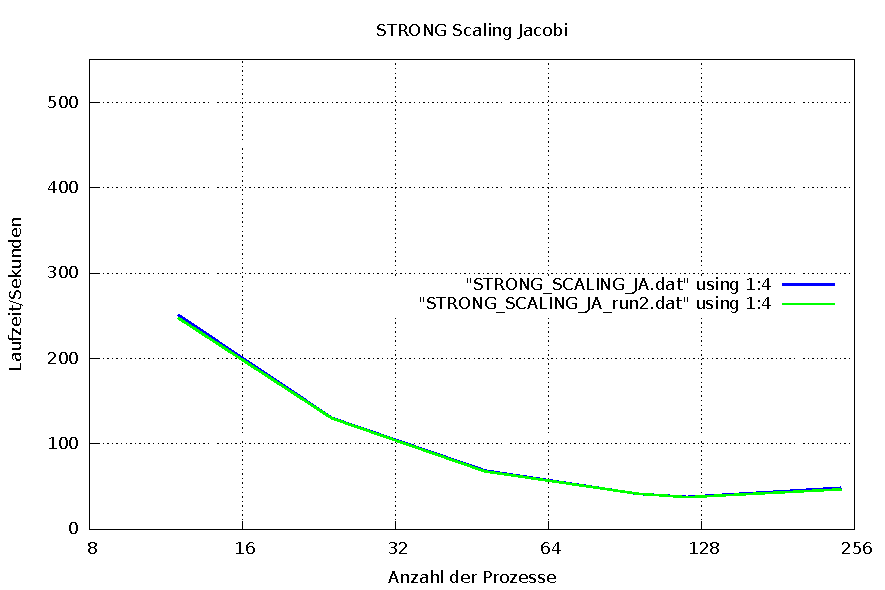
\includegraphics[scale=0.8]{img/STRONG_SCALING_JA_laufzeit.pdf}

Grundsätzlich ist hier bei steigender Prozesszahl ein schöner antiproportionaler Verlauf zu betrachten. Auch ein Blick in die Tabelle zeigt, dass unser Programm von 12-48 Prozessen gut skaliert, dies jedoch bei weiter steigender Prozesszahl abnimmt. Bei der Verdoppelung der Prozesse von 120 auf 240 gibt es gar eine Steigerung der Laufzeit um ca. 25\%. Hier steht die doppelt so große Prozesszahl der deutlich vermehrten Kommunikation entgegen, dies scheint auch den Vorteil des Hyperthreading zu verringern.

\subsection{Gauß-Seidel}
\begin{tabular}{|c|c|c|}
\hline 
Anzahl der Prozesse & Laufzeit in s & Laufzeit in s (2. Durchlauf) \\ 
\hline 
12 & 443.7 & 424.9 \\ 
\hline 
24 & 233.3 & 234.0 \\ 
\hline 
48 & 118.3 & 116.5 \\ 
\hline 
96 & 64.2 & 65.8 \\ 
\hline 
120 & 52.8 & 53.5 \\ 
\hline 
240 & 39.7 & 39.7 \\ 
\hline
\end{tabular} 

Wobei die Anzahl der genutzten Knoten stets $\frac{Anzahl Prozesse}{12}$ entspricht. Auch bei 240 Prozessen wurden jedoch 10 Knoten verwendet. Weiterhin wurden in jedem Lauf 960 Interlines verwendet.

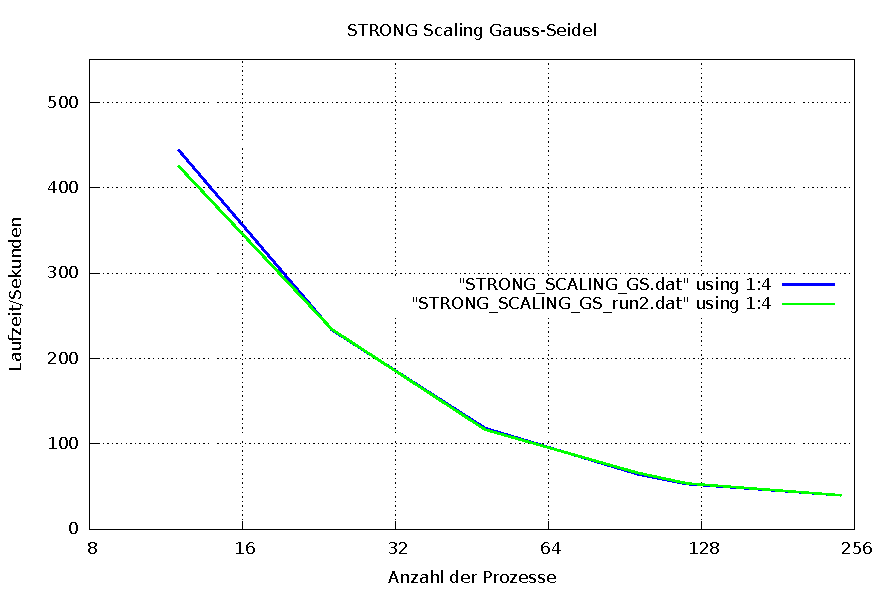
\includegraphics[scale=0.8]{img/STRONG_SCALING_GS_laufzeit.pdf}

Anders als die Implementation des Jacobi-Verfahrens skaliert das Gauß-Seidel-Verfahren auch beim letzten Verdoppelungsschritt von 120 auf 240 Prozesse. Allgemein ist hier ein besseres Skalierungsverhalten bis in größere Prozesszahlen zu beobachten. 

\section{Weak Scaling}
\subsection{Jacobi}
\begin{tabular}{|c|c|c|c|c|}
\hline 
Prozesse & Knoten & Interlines & Laufzeit in s & Laufzeit in s (2. Durchlauf) \\ 
\hline 
1 & 1 & 100 & 36.9 & 36.9 \\ 
\hline 
2 & 1 & 141 & 36.9 & 37.2 \\ 
\hline 
4 & 2 & 200 & 38.5 & 38.1 \\ 
\hline 
8 & 4 & 282 & 38.9 & 41.6 \\ 
\hline 
16 & 4 & 400 & 44.4 & 44.6 \\ 
\hline 
24 & 4 & 490 & 42.9 & 44.7 \\ 
\hline 
64 & 8 & 800 & 55.0 & 53.0 \\ 
\hline 
\end{tabular} 

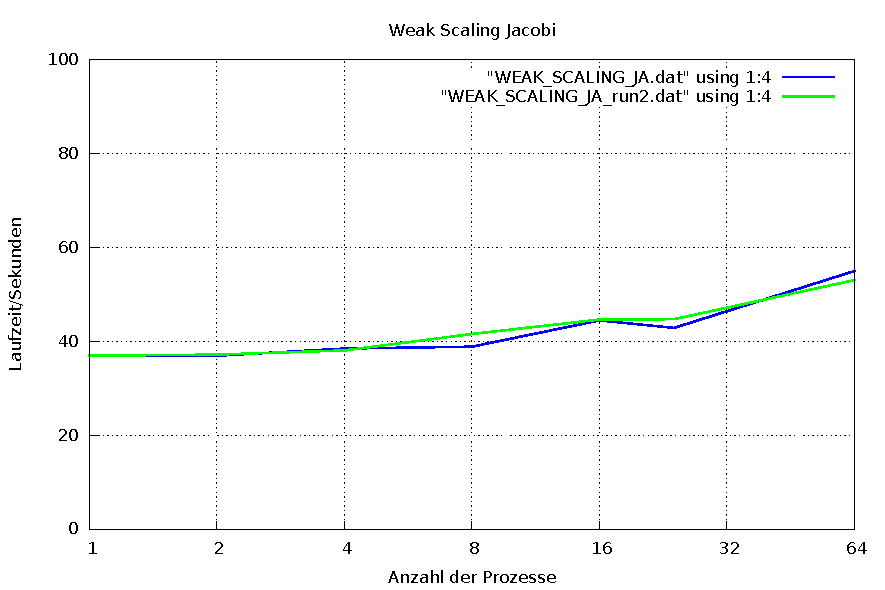
\includegraphics[scale=0.8]{img/WEAK_SCALING_JA_laufzeit.pdf}

Die Implementation des Jacobi-Verfahrens schlägt sich im Weak-Scaling gut. Bei steigender Prozesszahl und proportionaler Vergrößerung des zu berechnenden Problems steigt die Berechnungszeit nur leicht an (ca. Faktor 1.5 zwischen kleinstem und größtem Problem). 

\subsection{Gauß-Seidel}
\begin{tabular}{|c|c|c|c|c|}
\hline 
Prozesse & Knoten & Interlines & Laufzeit in s & Laufzeit in s (2. Durchlauf) \\ 
\hline 
1 & 1 & 100 & 37.4 & 37.3 \\ 
\hline 
2 & 1 & 141 & 74.5 & 73.7 \\ 
\hline 
4 & 2 & 200 & 75.3 & 77.6 \\ 
\hline 
8 & 4 & 282 & 76.35 & 78.9 \\ 
\hline 
16 & 4 & 400 & 85.0 & 77.9 \\ 
\hline 
24 & 4 & 490 & 77.6 & 79.5 \\ 
\hline 
64 & 8 & 800 & 92.0 & 91.8 \\ 
\hline 
\end{tabular} 

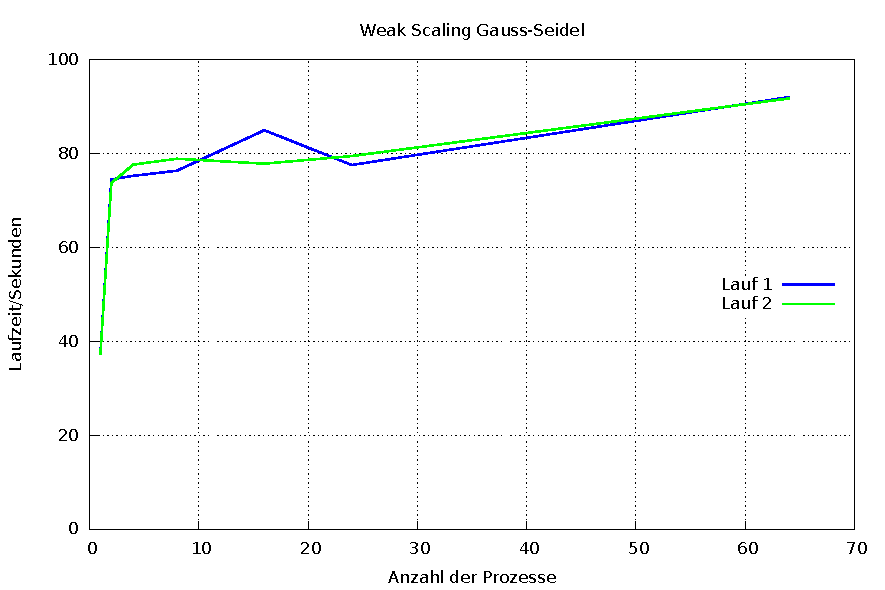
\includegraphics[scale=0.8]{img/WEAK_SCALING_GS_laufzeit.pdf}

Anders als im Jacobi-Verfahren skaliert die Implementation des Gauß-Seidel-Verfahrens nicht sonderlich gut. Bereits im ersten Schritt (verdoppelung der Problemgröße bei zwei Prozessen auf einem Knoten) beobachten wir eine Veroppelung der Laufzeit. Dies wird dadurch begründet sein, dass bei einem Prozess keinerlei Kommunikation statt findet, wobei bei zwei Prozessen die beiden Prozesse jeweils aufeinander warten müssen, bis sie weiter berechnen können, hierdurch entstehen natürlich Verzögerungen. Im weiteren Verlauf ist die Implementierung jedoch relativ stabil, lediglich bei sehr großen Problemgrößen bzw. Prozesszahlen steigt die Laufzeit wieder an.

\section{Kommunikation und Teilnutzung der Knoten}
\subsection{Jacobi}
\begin{tabular}{|c|c|c|}
\hline 
Knoten (je 10 Proz.) & Laufzeit in s & Laufzeit in s (2. Durchlauf) \\ 
\hline 
1 & 23.7 & 20.0 \\ 
\hline 
2 & 17.1 & 20.9 \\ 
\hline 
3 & 20.2 & 23.7 \\ 
\hline 
4 & 23.0 & 27.1 \\ 
\hline 
6 & 26.8 & 29.5 \\ 
\hline 
8 & 25.9 & 29.7 \\ 
\hline 
10 & 45.1 & 52.3 \\ 
\hline 
\end{tabular} 

Mit je 200 Interlines.

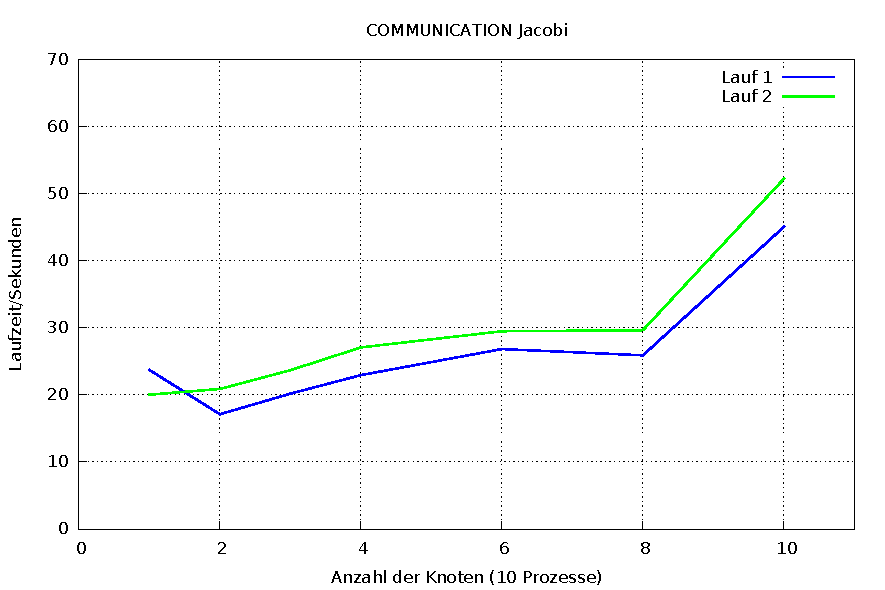
\includegraphics[scale=0.8]{img/COMMUNICATION_JA_laufzeit.pdf}

Da wir in dieser Problemstellung eine fixe Anzahl an Prozessen haben, nämlich zehn, und die Anzahl der verwendeten Knoten stets erhöhen steigt mit jeder Erhöhung der Knotenzahl die Zeit, welche für die Kommunikation benötigt wird drastisch an, denn Kommunikation zwischen zwei Rechnern ist deutlich langsamer als zwischen zwei Prozessen auf einem Knoten. Zwar steigt die Laufzeit nicht proportional zur Anzahl der Prozesse, jedoch ist ein nahezu lineares Wachstum zu betrachten.

\subsection{Gauß-Seidel}
\begin{tabular}{|c|c|c|}
\hline 
Knoten (je 10 Proz.) & Laufzeit in s & Laufzeit in s (2. Durchlauf) \\ 
\hline 
1 & 45.0 & 45.1 \\ 
\hline 
2 & 50.6 & 52.4 \\ 
\hline 
3 & 52.6 & 52.5 \\ 
\hline 
4 & 56.7 & 54.4 \\ 
\hline 
6 & 55.9 & 56.3 \\ 
\hline 
8 & 55.3 & 57.1 \\ 
\hline 
10 & 83.4 & 87.8 \\ 
\hline 
\end{tabular} 

Mit je 200 Interlines.

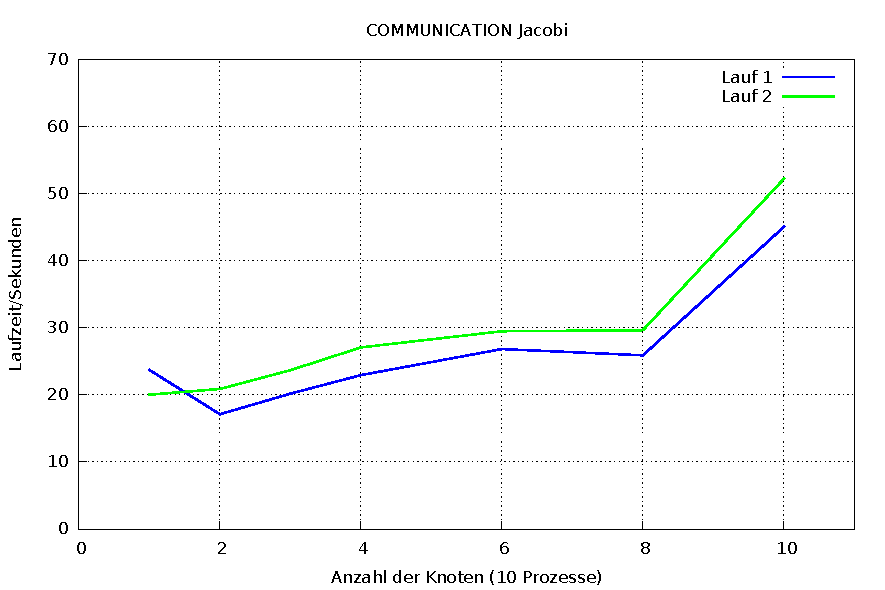
\includegraphics[scale=0.8]{img/COMMUNICATION_JA_laufzeit.pdf}

Gleiches ist auch beim Gauß-Seidel-Verfahren zu beobachten. Der Verlauf ist aus den selben Gründen wie beim Jacobi-Verfahren diesem sehr ähnlich. 

\end{document}